% Main Thesis File: This is the main file and it connects all the different parts of the thesis and compiles it into a single outcome file.

\documentclass[onecolumn, 12 pt, doublespace, fullpage, a4paper]{report}
\renewcommand{\baselinestretch}{1.75} % baseline stretch

% Packages
\usepackage{amssymb}
\usepackage{amsthm}
\usepackage[cmex10]{amsmath}
\usepackage{adjustbox} 
\usepackage{arabtex} 
\usepackage{academicons}
\usepackage{breakcites} 
\usepackage{color}
\usepackage{epsfig}
\usepackage{epstopdf}
\usepackage{etoolbox}
\usepackage{enumitem}
\usepackage{float}
\usepackage{fancyhdr}
\usepackage{graphicx}
%for \includegraphics[]{picturename.filetype} command
\usepackage{graphics}
%\usepackage[breaklinks]{hyperref} % if you want to highlight the links
%\usepackage[hidelinks]{hyperref}
\usepackage{latexsym,amsfonts}
\usepackage{longtable}
\usepackage{listings}
\usepackage{lscape} 
\usepackage{lipsum}
\usepackage{multirow}             
\usepackage{pdfpages}
\usepackage[figuresright]{rotating} 
\usepackage{sectsty}
\usepackage{setspace}
\usepackage{subfigure}
\usepackage{textcomp}
\usepackage{utf8} 
\usepackage[hyphens]{url} 
\usepackage{wrapfig} 
\usepackage{wasysym} 
\usepackage{xcolor}
\usepackage[table,xcdraw]{xcolor}
%listset command to insert code [from Stack Overflow]%
\definecolor{dkgreen}{rgb}{0,0.6,0}
\definecolor{gray}{rgb}{0.5,0.5,0.5}
\definecolor{mauve}{rgb}{0.58,0,0.82}

\lstset{frame=tb,
  language=Mathematica,
  aboveskip=3mm,
  belowskip=3mm,
  showstringspaces=false,
  columns=flexible,
  basicstyle={\small\ttfamily},
  numbers=none,
  numberstyle=\tiny\color{gray},
  keywordstyle=\color{blue},
  commentstyle=\color{dkgreen},
  stringstyle=\color{mauve},
  breaklines=true,
  breakatwhitespace=true,
  tabsize=3
}

% you can define your most used synonyms/acronyms
\def\KAUST {King Abdullah University of Science and Technology}
\def\dg{$^\circ$}		 % for degree celcius
\def\2{$^2$}			 % for raised to power 2
\def\3{$^3$}			 % for raised to power 3
\def\-2{$^{-2}$}		 % for raised to power -2
\def\-3{$^{-3}$}		 % for raised to power -2
\def\-1{$^{-1}$}		 % for raised to power -1
\def\h{W.m$^{-2}$K$^{-1}$}
\def\hh{kJ.kg$^{-1}$}
\def\hfg{kJ.kg$^{-1}$}
\def\ss{kJ.kg$^{-1}$K$^{-1}$}
\def\Q{W.m$^{-2}$}
\def\mone {$^{-1}$}
\def\mtwo {$^{-2}$}
\def\um{$\mu m$}
\def\kwhm{kWh.m$ ^{-3} $}
\def\LMH{kg.m$^{-2}$h$^{-1}$}


% Changing chapters' headings and subheadings to size 14
\chapterfont{\fontsize{14}{15}\selectfont}   % font size and baseline stretch
\sectionfont{\fontsize{14}{15}\selectfont}
\subsectionfont{\fontsize{14}{15}\selectfont}
\subsubsectionfont{\fontsize{14}{15}\selectfont}

       
\pagestyle{fancy} % adds a line at the top of every page, except title-page
\fancyhead{} \fancyfoot{} % for header and footer
\fancyfoot[CO,CE]{\thepage}    % center odd and even page number

%centering the page numbers with text body
\fancyheadoffset[L]{0.01mm}
\renewcommand{\headrulewidth}{0pt}


%The following code changes the empty vertical space above a new chapter title. It sets it from 50pt to 20pt
\makeatletter
\patchcmd{\@makechapterhead}{50\p@}{20pt}{}{}
\patchcmd{\@makeschapterhead}{50\p@}{20pt}{}{}
\makeatother
%end of modification



% The following code redefines the plain pagestyle with the objective of moving the page number from the bottom to the top of the page. This only affects new chapter pages.
\fancypagestyle{plain}{
\fancyhf{} %clear all header and footer fields
\fancyhead[C]{\thepage} %puts number on top center of the page
\renewcommand{\headrulewidth}{0pt}
\renewcommand{\footrulewidth}{0pt}}
%ending of plain pagestyle modification.




% ### Nomenclature, List of Abbreviations and List of Symbols 
   \usepackage{ifthen,xkeyval,xfor,amsgen}
   \usepackage[acronym,toc, nogroupskip]{glossaries}
   \newglossary[slg]{symbols}{syi}{sbl}{List of Symbols}
 
   \makeglossaries
   
   
% #### Symbols ####
\newglossaryentry{symb:Pi}{
name=$\pi$, type=symbols,
description=A mathematical constant whose value is the ratio of any circle's circumference to its diameter,
sort=symbolpi
}

\newglossaryentry{symb:Phi}{
name=$\varphi$, type=symbols,
description=An angle,
sort=symbolphi
}

\newglossaryentry{symb:Lambda}{
name=$\lambda$, type=symbols,
description=Lambda indicates usually an eigenvalue in linear algebra,
sort=symbollambda
}

% #### Abbreviations ####
\newacronym{toc}{ToC}{Table of Contents}
\newacronym{los}{LoS}{List of Symbols}
\newacronym{loa}{LoA}{List of Abbreviations}
\newacronym{phd}{PhD}{Doctoral}
\newacronym{MS}{MS}{Masters}
\newacronym{M$}{MS}{Microsoft}
\newacronym{CD}{CD}{Compact Disc}
\newacronym{kaust}{KAUST}{King Abdullah University of Science and Technology}

%An acronym with a glossary entry
\newacronym{AD}{AD}{Active Directory\protect\glsadd{glos:AD}}



% #### Nomenclature terms ####
\newglossaryentry{glos:AD}{
name=Active Directory,
description={Active Directory is the directory service for Windows based networks, that allows central organization and administration of any network resource. It allows a single-sign-on concept independent from network topologies or network protocols. As a prerequisite you need a Windows Server acting as Domain Controller. This computer stores all necessary data, e.g.~usernames and corresponding passwords}
}

\newglossaryentry{glos:RespF}{name=response file, description={A file 
that allows unattended software installation}}


   % Run the following three lines in the command line to get the lists
%makeindex -s Thesis.ist -t Thesis.alg -o Thesis.acr Thesis.acn
%makeindex -s Thesis.ist -t Thesis.slg -o Thesis.syi Thesis.sbl
%makeindex -s Thesis.ist -t Thesis.glg -o Thesis.gls Thesis.glo

% ### End of addition




% Modified commands
\newcommand{\Tab}{\hspace{2ex}}
\usepackage[lmargin=40mm, rmargin=25mm, vmargin=25mm, headsep=2.5mm]{geometry}
\newcommand{\mathsym}[1]{{}}
\newcommand{\unicode}[1]{{}}
\renewcommand{\thechapter}{\arabic{chapter}}
\renewcommand\bibname{\centering BIBLIOGRAPHY}
%\newcommand{\orcid}[1]{\href{https://orcid.org/#1}{\textcolor[HTML]{A6CE39}{\aiOrcid}}}
\newcommand{\orcid}{
\includegraphics[width=8pt]{ORCID}} % ORCID ID


\begin{document}

% $$$$$$$$$$$$$$$$$  Start of Thesis Front matter   $$$$$$$$$$$$$$

%\vspace{10mm}  % vertical space
\thispagestyle{empty}
\addvspace{5mm}  % vertical space until length

%$$$$$$$$$$$$$$$$$$$$$$$$$$$$$$$$$$$$$$$$$$$$$$$$$$$$$$$$$$$$$$$$$$$$$$$$$$$$$$$$$

% make the title page
\begin{center}
\begin{doublespace}
{\textbf{{\large A Quantitative Analysis on the Distance Traversed by Hikers}}}%\vfill % Write your thesis title
\end{doublespace}

\vspace{10mm}
{A Project By}\\
{Sonny Luong}\\
{Cory Suzuki}\\
{December 16, 2023}%\vfill

\vspace{30mm}

{ In Partial Fulfillment of the Requirements}\\[12pt]
{ For Course Completion and the Advancement to Candidacy}\\[12pt]
\vfill
{California State University, Long Beach }\\
{California, United States of America}\\
{Dr. Tianni Zhou}
\vfill

\end{center}
% end of title page
%$$$$$$$$$$$$$$$$$$$$$$$$$$$$$$$$$$$$$$$$$$$$$$$$$$$$$$$$$$$$$$$$$$$$$$$$$$$$$$$$$
\newpage

\chaptertitlefont{\fontsize{14}{15}\selectfont\centering}  



% Abstract File
% Do not remove centering environment below
\begin{center}

\end{center}

\begin{center}
{{\bf\fontsize{14pt}{14.5pt}\selectfont \uppercase{ABSTRACT}}}
\end{center}

\doublespacing
\addcontentsline{toc}{chapter}{Abstract}



\begin{center}
	\begin{doublespace}
%{\fontsize{14pt}{14.5pt}\selectfont {Applications of Cubic Spline Interpolation On Functions in Normed Spaces}}\\
		%{\fontsize{14pt}{14.5pt}\selectfont {Cory Suzuki}}\\
%		{\fontsize{12pt}{12.5pt}\selectfont {Ph.D. Year}}\\
	\end{doublespace}
\end{center}


In this paper, we provide a detailed experimental investigation of the physical activity performance of hikers. The response variable of primary interest is the number of miles a hiker can hike within a sixty-minute time frame. The variable factors to be blocked will be temperature which is measured in degrees and humidity level which is measured in percent. For this experiment, since the temperature and humidity level are of little interest, these nuisance factors will be blocked using a Latin Square design of size $4$ with $3$ replications. From the analysis of the data, we conclude that temperatures 70 degrees Fahrenheit and 75 degrees Fahrenheit are statistically significant. For humidity levels in percentages, humidity levels $5\%$, $10\%$, $15\%$ are statistically significant. 
  % include your abstract file


\include{Acknowledgment}  % include your Acknowledgement file


\begin{onehalfspacing}%To make the table of contents, figures, and tables single spaced, as required by the formatting guidelines, pg. 24.

%\renewcommand{\contentsname}{\textbf{{\large TABLE OF CONTENTS}}}
\tableofcontents
% Maybe we don't need this blank page.
%\cleardoublepage

\printglossary[type=\acronymtype,style=long3col, title=\centerline{LIST OF ABBREVIATIONS}, toctitle=List of Abbreviations, nonumberlist=true] 

\printglossary[type=symbols,style=long3col, title=\centerline{LIST OF SYMBOLS}, toctitle=List of Symbols, nonumberlist=true]


\end{onehalfspacing}
% \printglossary[style=altlist,title=Nomenclature, toctitle=Nomenclature, nonumberlist=true] 

% $$$$$$$$$$$$$$$$$  Thesis front matter ends   $$$$$$$$$$$$$$



% $$$$$$$$$$$$$$$$$  include your separate chapters   $$$$$$$$$$$$$$
% Remove the centering of chapter name.
\chaptertitlefont{\fontsize{14}{15}\selectfont}  % <------ Add this line


% Chapter 2 File

\chapter{Introduction}
\label{chapter1}
\thispagestyle{empty}

\section{Motivation for Research: Why is the Performance of Hikers Important?}
Hiking is an excellent recreational activity that any individual can enjoy regardless of their hiking skill level. It is often nice to experience the outdoors from a new perspective and to see the local wildlife as one climbs rocky mountains covered in boulders or traverses through the extreme weather of desert landscapes. However, hiking does come with certain risks and there are numerous factors that can affect an individual's hike. For example, the weather can be too hot or too cold, and that can affect respiratory function which is required for long-distance hikes. The altitude of a mountain can also wear out hikers who are less experienced.
\\\\
More than often, hikers need to check the humidity percentage as it is a factor that accelerates your body's dehydration. If the trail is located in the mountains or near coastlines, the humidity level will be higher than the humidity in typical urban and suburban areas. Many hiking safety guides such as the site \emph{Hiking with Shawn}, warn potential hikers of dehydration due to the increased amount of bodily perspiration as a result of both high temperatures and high humidity levels \cite{key1}. The safety of both experienced and inexperienced hikers is important and above all, a guaranteed way to provide the adventure and excitement of experiencing the great outdoors, which proposes the question: Can we construct and conduct an experiment to analyze and draw meaningful statistical conclusions to facilitate in the development of better gear and technology for hikers? The analysis discussed in further detail in this paper provides a meaningful answer to this question.

% Chapter 3 File

\chapter{Statistical Modeling and Methodology}
\label{chapter2}
\thispagestyle{empty}

\section{Latin Square Model and Specifications}
The Replicated Latin Square model (Case I) of size $p=4$ is a type of randomized complete block design that contains letters from the Latin alphabet in which each letter represents a treatment, which is the distance covered by hikers within a sixty-minute interval in the conducted experiment, each of the letters are randomly permuted and no single letter is repeated in the same row and column. This is synonymous with the design of Sudoku puzzles where each column and row entry is unique. The experiment considers three replications of the standard Latin Square design by fixing the nuisance factor levels and replicating the experiment over a given number of times. Three replications spread throughout a three consecutive day basis were considered. According to the Pennsylvania State University's Experimental Design and Analysis online textbook, this experiment is orthogonal due to the unique random permutation property of the Latin letters previously mentioned \cite{key2}. This allows the design to be easier and cleaner to analyze since interaction effects are not considered as relevant in the experiment. The model in terms of mathematical notation is given by:\\
\centerline{$y_{ijkl} = \mu + \tau_{i} + \rho_{j} + \beta_{k} + \delta_{l} + \epsilon_{ijkl}$}\\
\centerline{$i = 1,2,3,4 \\
j = 1,2,3,4 \\
k = 1,2,3,4\\
l = 1,2,3$}\\
Note that in this model, the iteration index j is dependent on i and k, which is denoted by j = d(i,k). This is the specific model for our experiment since the experiment will include four levels each of temperature and humidity respectively. The Greek letter $\mu$ denotes the overall mean distance within the sixty-minute time period. The next term in the above equation, denoted as $\tau_{i}$ is the ith "...". The following term is $\rho_{j}$ which is the jth level of the temperature block variable. $\beta_{k}$ is the kth level of the humidity percentage block variable. The term $\delta_{l}$ represents the lth replicate of the experiment in which the experiment was repeated for three consecutive days in which the same levels of both temperature and humidity were measured. Lastly, $\epsilon_{ijkl}$ is the random error term of the Latin Square model.\\\\
\section{Assumptions of the Latin Square Statistical Model}
In this section, the required assumptions and appropriate hypothesis tests are provided to better inform the reader of how the statistical analysis will be conducted. In this model, we assume that:\\
\centerline{$1. \sum_{i}^{4} \tau_{i} = 0$}
\centerline{$2. \sum_{j}^{4} \rho_{j} = 0$}
\centerline{$3. \sum_{k}^{4} \beta_{k} = 0$}
\centerline{$4. \sum_{l}^{3} \delta_{l} = 0$}
\centerline{$5. \epsilon_{ijkl} \overset{iid}{\sim} N(0,\sigma^2) $}\\\\
These assumptions indicate that the summation of each of the respective effects should be equal to $0$ and that the random error term of the Latin Squares model should be independently and identically distributed with a Normal distribution of mean $0$ and variance $\sigma^2$.\\\\
\section{Hypothesis Test of the Latin Squares Model}
For the analysis of the experiment, we consider the following set of hypotheses and the F test ratios\cite{key3}:\\
\centerline{$H_o: \tau_{i} = 0$}\newline
\centerline{$H_a: \tau_{i} \neq 0$}\newline
\centerline{$H_o: \rho_{j} = 0$}\newline
\centerline{$H_a: \rho_{j} \neq 0$}\newline
\centerline{$H_o: \beta_{k} = 0$}\newline
\centerline{$H_a: \beta_{k} \neq 0$}\newline
\centerline{$H_o: \delta_{l} = 0$}\newline
\centerline{$H_a: \delta_{l} \neq 0$}\newline
\centerline{$F^* = \frac{MS_{trt}}{MS_{E}}$}\newline
\centerline{$F^* = \frac{MS_{row}}{MS_{E}}$}\newline
\centerline{$F^* = \frac{MS_{col}}{MS_{E}}$}\newline
\centerline{$F^* = \frac{MS_{rep}}{MS_{E}}$}\\
The F test ratio value $F^*$ is the mean squared value for the treatments divided by the mean squared value for the error within the model. The other F test ratios are calculated similarly with the respective mean square values of each model component. The calculations of the mean square values will be elaborated on in the following section. The null hypothesis produces the inference that the mean treatment effects are insignificant, while the alternative hypothesis produces the inference that the mean treatment effects differ. For this experiment, the significance level is set to the default $\alpha = 0.05$ when the hypothesis test is conducted using the data from the analysis of variance (ANOVA) table.\\
We reject the null hypothesis $H_o$ if the F test ratio value is greater than the F critical value. This leads to the conclusion that the mean distance effects are statistically significant, meanwhile, if the F test ratio value is less than the F critical value, the appropriate conclusion is that we fail to reject the null hypothesis $H_o$ and conclude that the mean distance effects are statistically insignificant. The full ANOVA table that was outputted from the computer is provided in the appendix section.

\section{Estimation of Effects and Generalization of the Replicated Latin Squares ANOVA Table}
The effects from the generalized linear model can be estimated using the following formulas:\\
\centerline{$\hat{\mu} = \overline{y}....$}\newline
\centerline{$\hat{\tau_{i}} = \overline{y}_{i...} - \overline{y}_{....}$}\newline
\centerline{$\hat{\rho_{j}} = \overline{y}_{.j..} - \overline{y}_{....}$}\newline
\centerline{$\hat{\beta_{k}} = \overline{y}_{..k.} - \overline{y}_{....}$}\newline
\centerline{$\hat{\delta_{l}} = \overline{y}_{...l} - \overline{y}_{....}$}\\
The estimate for the overall mean distance effect is the grand mean of the data set which is calculated by adding all the observations in the data and dividing by the total number of observations. The treatment effect estimate is calculated by subtracting the mean of the ith treatment group by the grand mean. Similarly, the temperature block effect is calculated by calculating the difference between the jth row average and the grand mean. For the humidity level block effect, the difference between the kth column average and the grand mean is calculated. Finally, the estimate for the replicate day effect is found by subtracting the lth replicate mean by the grand mean. Note that these averages are taken of the data collected in the experiment being analyzed. We provide these estimates in the respective appendix section. Provided below is a brief summary of the replicated Latin Square (Case I) design ANOVA table. In this table, $p$ represents the size of the Latin Square, $n$ correlates to the number of replications, and the total sum of squares of the data is denoted by $SS_{T}$. For notation convenience and ease, these are the conventional symbols that will be used when analyzing the calculations from the computer output in the following chapter.\\
\begin{figure}[htp]
    \centering
    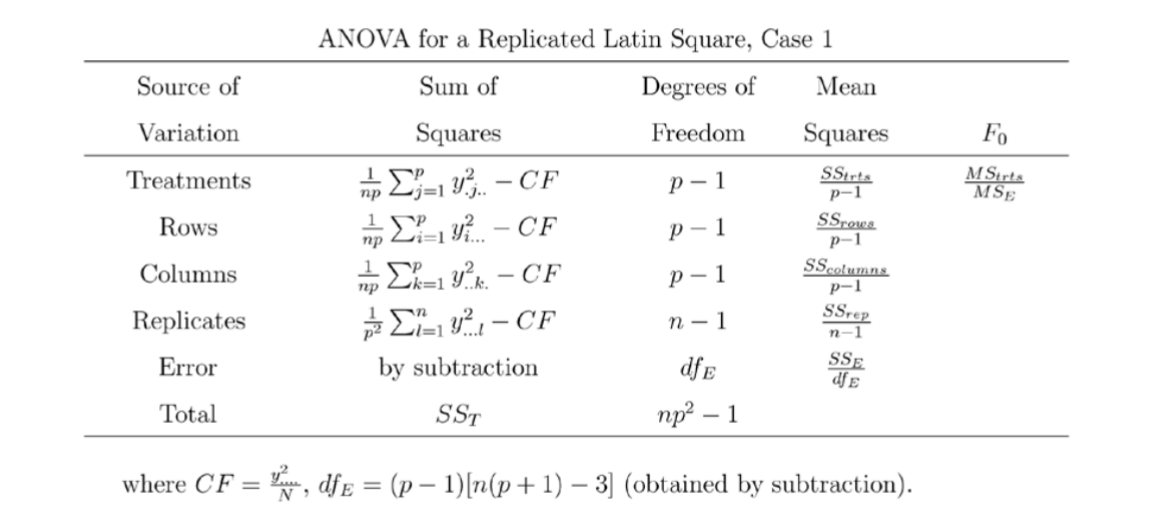
\includegraphics[width=150mm]{ANOVA_RepLS.png}
    \caption{The generalized Analysis of Variance table for the Replicated Latin Square Design (Case I)}
    \label{fig:ANOVA_Repls}
\end{figure}

% Chapter 4 File

\chapter{Experiment Analysis and Results}
\label{chapter3}
\thispagestyle{empty}

\section{Numerical Estimation of Parameters}
We will continue by providing the numerical estimates of the parameters in the model used for the experiment. The estimates for each model term are given by:\\
\centerline{$\hat{\mu} = 5.4583$}
\centerline{$\hat{\tau_{i}} = 60.0417$}
\centerline{$\hat{\rho_{j}} = 60.0417$}
\centerline{$\hat{\beta_{k}} = 60.0417$}
\centerline{$\hat{\delta_{l}} = 81.875$}\\
It is interesting to remark that the treatment, row, and column parameter estimates are the same because of the orthogonality property the Replicated Latin Square design follows. Each of the indexes is the same as well due to the square's size of $4 \times 4$. From these estimates, it can be observed that the replicates seem to be the portion of the model that contributes most to the overall mean distance traversed by hikers, while the treatment, row, and column means indicate little contribution to the overall mean effect. These inferences will further be tested by the following ANOVA table and confidence intervals.

\section{Analysis of Variance Results}
In this section, we analyze the ANOVA table which was produced using the Microsoft Excel software to verify the hand calculation work and the formulas provided from the Stat 530 lecture notes \cite{key3}. The ANOVA table can be found in Appendix A. The sum of squares for temperature seems to be larger than the other sum of square quantities, so it can be suspected that there may be significant differences between the humidity level means. This conclusion will be supported in the section that discusses the analysis of the confidence intervals.\\\\
From the ANOVA table, it is imperative to note that to test the treatment effects hypothesis previously mentioned, the F test ratio is compared to the F critical value. They are given as:\\
\centerline{$F^{*} = \frac{MS_{trt}}{MS_{E}} = 0.3545$}\newline
\centerline{$F^{*} = \frac{MS_{row}}{MS_{E}} = 0.8423$}\newline
\centerline{$F^{*} = \frac{MS_{col}}{MS_{E}} = 77.4979$}\newline
\centerline{$F^{*} = \frac{MS_{rep}}{MS_{E}} = 0.8040$}\newline
\centerline{$F_{0.05,4,36} = 2.634$}\\
So by the lecture notes provided by the Stat 530 course instructor, we fail to reject $H_o$ and conclude that the mean treatment, row, and replication effects are not statistically significant, which is supported by the conclusions from the parameter estimates.
However, we reject $H_{o}$ and conclude that the mean column effect is statistically significant since its F test ratio is significantly larger than the provided F critical value. This implies that the temperature-blocking factor may be the most significant in providing information about the average hiker's physical performance. To further support this result, we proceed by constructing $95\%$ confidence intervals for the pairwise difference of means for the temperature and humidity level blocking factors.

\section{Post-ANOVA Analysis using the Method of Confidence Intervals}
After conducting the main analysis of the hiking data, it is also a wise decision to conduct some additional analysis in the form of confidence intervals for the difference in factor means. We define this contrast as:\\
\centerline{$|\mu_{i}... - \mu_{i...'}|$}\\
where we take the difference of means from two different factor levels. The intention behind this section of this experiment is to further investigate if there is a difference in mean effects to support the statistical conclusion reached in the previous section. The respective confidence intervals for both the temperature and humidity levels are provided below:\\
\centerline{$-0.1497 \leq (\mu_{1...} - \mu_{2...}) \leq 1.3297$}\newline
\centerline{$-0.5497 \leq (\mu_{1...} - \mu_{3...}) \leq 0.9297$}\newline
\centerline{$2.2403 \leq (\mu_{1...} - \mu_{4...}) \leq 3.7197$}\newline
\centerline{$-0.3397 \leq (\mu_{2...} - \mu_{3...}) \leq 1.1397$}\newline
\centerline{$2.8303 \leq (\mu_{2...} - \mu_{4...}) \leq 4.3097$}\newline
\centerline{$2.4303 \leq (\mu_{3...} - \mu_{4...}) \leq 3.9097$}\\\\
\centerline{$9.8503 \leq (\mu_{.1..} - \mu_{.2..}) \leq 11.3297$}\newline
\centerline{$24.1103 \leq (\mu_{.1..} - \mu_{.3..}) \leq 25.5897$}\newline
\centerline{$35.0203 \leq (\mu_{.1..} - \mu_{.4..}) \leq 36.4997$}\newline
\centerline{$13.5203 \leq (\mu_{.2..} - \mu_{.3..}) \leq 14.9997$}\newline
\centerline{$24.4303 \leq (\mu_{.2..} - \mu_{.4..}) \leq 25.9097$}\newline
\centerline{$10.1703 \leq (\mu_{.3..} - \mu_{.4..}) \leq 11.6497$}\\

The first six confidence intervals are for the humidity levels factor while the six other confidence intervals describe the temperature level factors. From these intervals, we are $95\%$ confident that the temperatures 70 degrees Fahrenheit and 75 degrees Fahrenheit are statistically significant. For humidity levels in percentages, humidity levels $5\%$, $10\%$, $15\%$ are statistically significant. These conclusions are supported by the presence of $0$ being within the appropriate confidence intervals. 

% Conclusion File

\chapter{Concluding Remarks}
\thispagestyle{empty}
\section{Summary}

In this experiment, we investigated the physical performance of hikers affected by two blocking variables, in which temperature and humidity levels were chosen. The Analysis of Variance concludes that temperature plays the most significant role in hiking. 

In addition, the post-ANOVA analysis supported this conclusion further by showing that for temperature, temperatures 70 degrees Fahrenheit and 75 degrees Fahrenheit are statistically significant. For humidity levels in percentages, humidity levels $5\%$, $10\%$, $15\%$ are statistically significant. These conclusions mean that higher temperatures are detrimental to a given hiker's health and physical endurance. Therefore, a good recommendation to solve this issue and to decrease the negative effects of high temperatures is to advocate widespread hydration drinks or the production of specialized shirts with cold packs that can cool hikers.

If future work is done on the replicated Latin Square (Case I) design with the field data collected, one potential improvement that can be made to improve the robustness of the analysis is to provide more replications of the experiment and consider higher levels of both temperature and humidity. For example, further analysis can be done with $p>4$ if more data is collected, and our conclusion may change due to the variation in the distances traversed since different hikers attain different physical activity levels. This would be a more interesting experiment, although a more laborious one that may yield intriguing results. We have the hopeful intention that this experiment will provide some insight on how to improve the safety of prospective adventurers and hikers.


% $$$$$$$$$$$$$$$$$  Reference style  Starts $$$$$$$$$$$$$$

\begin{onehalfspacing}
	\renewcommand*\bibname{\centerline{REFERENCES}} 
    \phantomsection
	\addcontentsline{toc}{chapter}{References}
	\newcommand{\BIBdecl}{\setlength{\itemsep}{0pt}}%To control space between bibliography entries
		\bibliographystyle{plain}
		\bibliography{References}
\end{onehalfspacing}

% $$$$$$$$$$$$$$$$$  Reference style Ends  $$$$$$$$$$$$$$


% $$$$$$$$$$$$$$$$$  include Appendices   $$$$$$$$$$$$$$

\appendix
		\newpage
		\begingroup
			\let\cleardoublepage\clearpage
			\begin{center}
			\vspace*{2\baselineskip}
			{ \textbf{{\large APPENDICES}}} 
            % Fixes the numbering of "new" section created with "\addcontentsline."
            % You need to add the "\phantomsection" before *every* "\addcontentsline."
            %\clearpage
            \phantomsection
			\addcontentsline{toc}{chapter}{Appendices} 
			\end{center}
            %\clearpage
            
% Appendix A File

\refstepcounter{chapter}%
\chapter*{\thechapter \quad ANOVA Table}
\label{appendixA}

\section{Replicated Latin Squares (Case I)}
\begin{figure}[htp]
    \centering
    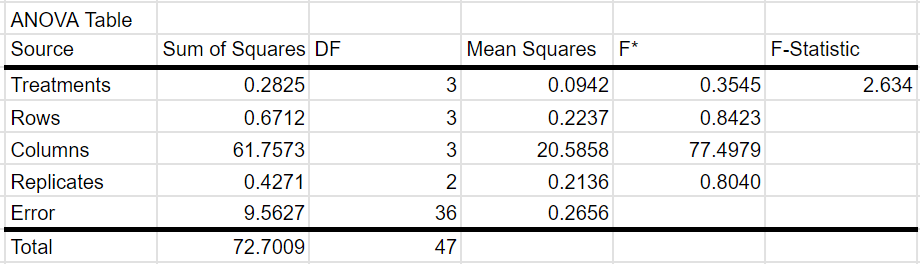
\includegraphics[width=150mm]{true_anova_stat530.png}
    \caption{The ANOVA table verified through the software application Microsoft Excel.}
    \label{fig:ANOVA}
\end{figure}

\begin{figure}[htp]
    \centering
    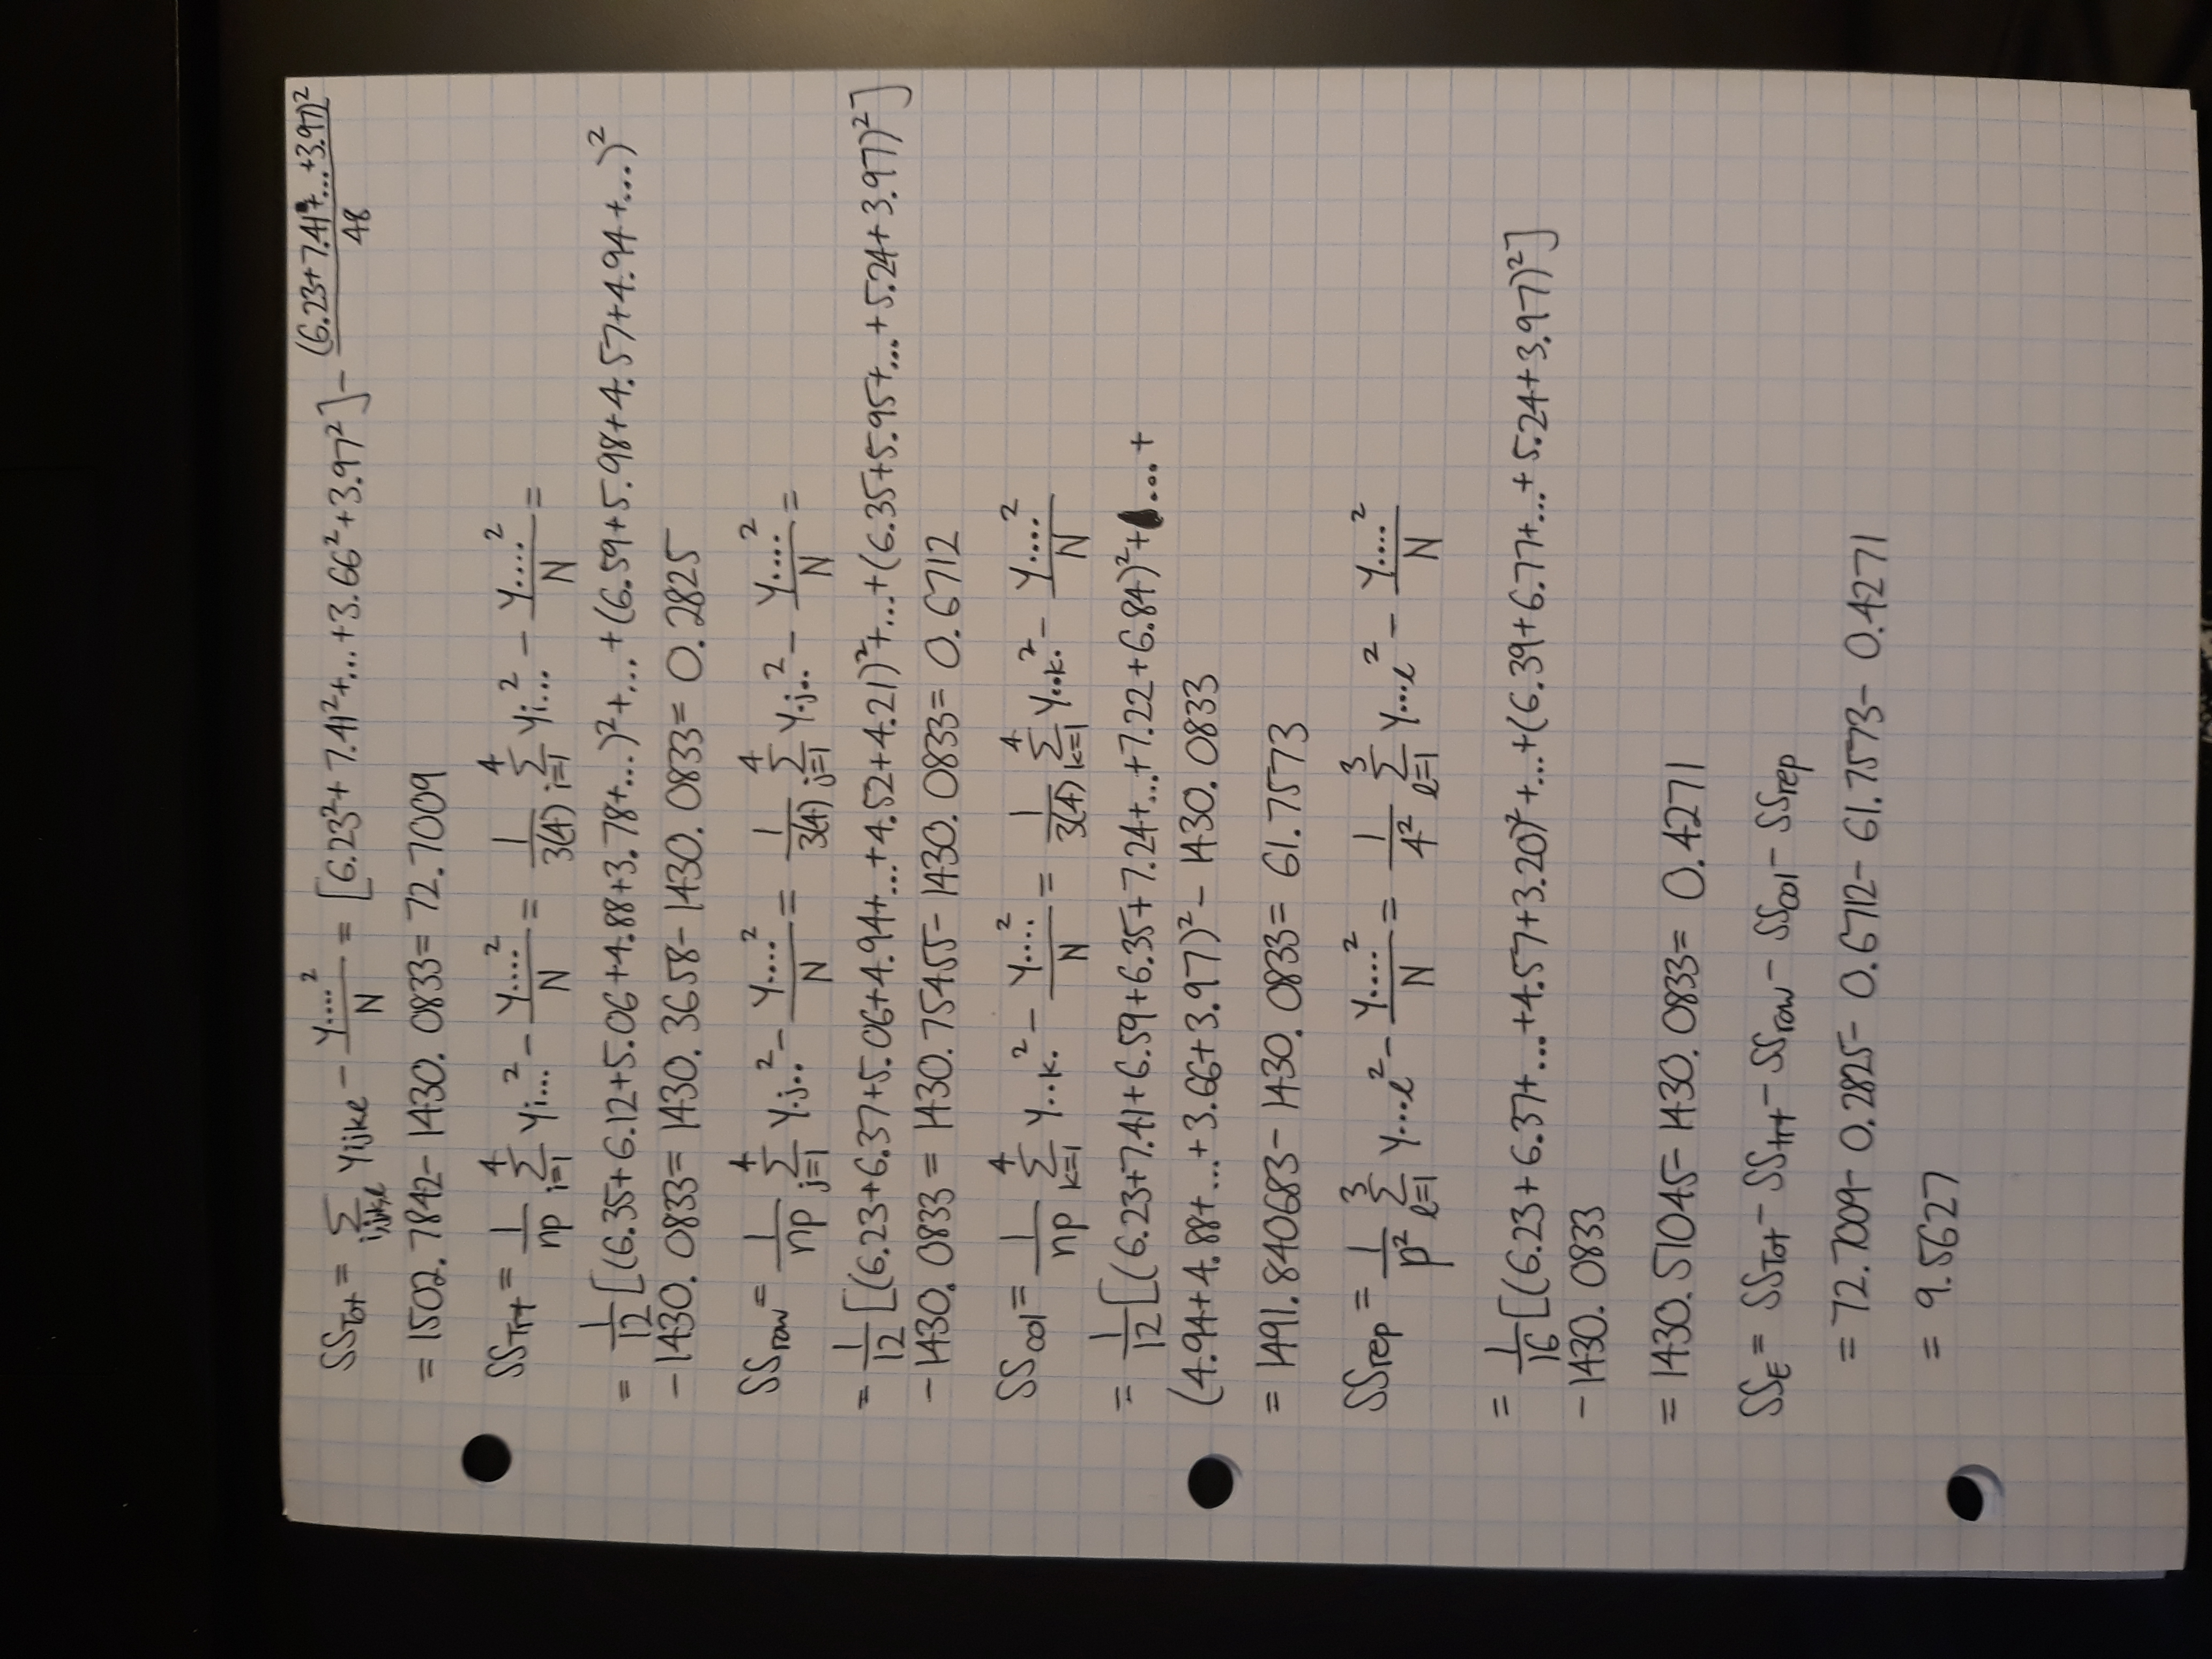
\includegraphics[width=150mm, angle=270]{handwork.jpg}
    \caption{The ANOVA table's sum of squares calculations done by hand.}
    \label{fig:ANOVA}
\end{figure}
            
% Appendix B File

\refstepcounter{chapter}%
\chapter*{\thechapter \quad Raw Hiking data}
\label{appendixB}

\section{Collection of Raw Data}
\begin{figure}[htp]
    \centering
    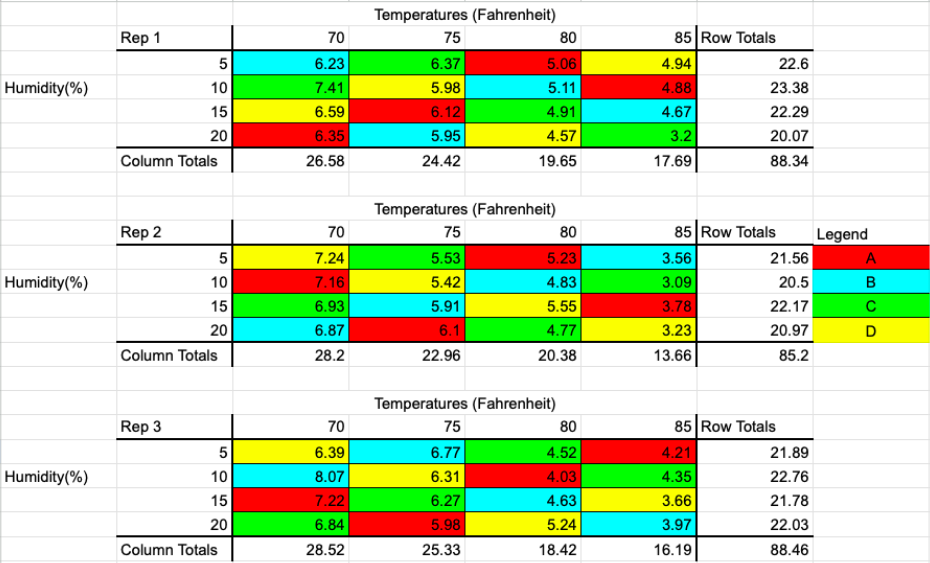
\includegraphics[width=150mm, origin=c]{530_proj_RawData.png}
    \caption{The raw data collected from the hikers, Cory and Sonny. Provided are also the random permutations of the Latin letters and their corresponding values measured in miles.}
    \label{fig:Raw Data}
\end{figure}

		\endgroup
% $$$$$$$$$$$$$$$$$  Appendix ends  $$$$$$$$$$$$$$

\end{document}

